% !TEX root = ../main.tex
\subsection{The Galaxy Sample}
The galaxies selected analysed in this paper are the 198 galaxies from \Lingard. These are a subset of the \textit{stellar mass-complete sample} in \citet{2017MNRAS.472.2263H}, a sample of low-redshift face-on spiral galaxies selected using data from the NASA-Sloan Atlas \citep{2011AJ....142...31B} and Galaxy Zoo 2 \citep{Willett2013:1308.3496v2}.

We combine classifications of galaxies which were repeated in the \textit{validation subset} with the original classifications. Clustering of drawn spiral arms and cleaning of points was then performed as detailed in \Lingard. We remove any galaxies for which fewer than two spiral arms were identified \comment{why exclude one-armed?}. This results in a hierarchical data structure of 91 galaxies, 211 spiral arms and 215,678 points.

Spiral arm points are deprojected to a face-on orientation using the disk inclination and position angle obtained through photometric model fitting performed in \Lingard. We scale the deprojected point radii to have unit variance, to aid chain convergence.

\subsection{Bayesian modelling of spiral arms in \textit{Galaxy Builder}}

We model a spiral arm as a logarithmic spiral, described by

\begin{equation}
r_\mathrm{arm} = \exp\left[\theta_\mathrm{arm}\tan\phi_\mathrm{arm} + c_\mathrm{arm}\right].
\end{equation}

Assume the pitch angle of a galaxy's spiral arms are drawn from a Normal distribution, truncated between 0 and 90 degrees, centred on some value we will call the galaxy's pitch angle, $\phi_\mathrm{gal}$. This dispersion in arm pitch angle has some measure of spread, $\sigma_\mathrm{gal}$, which we will assume is the same in galaxies:

\begin{equation}
\phi_\mathrm{arm} \sim \mathrm{TruncatedNormal}(\phi_\mathrm{gal}, \sigma_\mathrm{gal}, \mathrm{min}=0, \mathrm{max}=90).
\end{equation}

We choose hyperpriors on $\phi_\mathrm{gal}$ and $\sigma_\mathrm{gal}$ of

\begin{align}
  \phi_\mathrm{gal} &\sim \mathrm{Uniform}(\mathrm{min}=0, \mathrm{max}=90),\\
  \sigma_\mathrm{gal} &\sim \mathrm{InverseGamma}(\alpha=2,\,\beta=20).
\end{align}

We also have the offset parameter $c$, and a measure of radial uncertainty $\sigma_r$:

\begin{align}
  c_\mathrm{arm} &\sim \mathrm{Cauchy}(\alpha=0,\,\beta=10),\\
  \sigma_r &\sim \mathrm{HalfCauchy}(\beta=0.2).
\end{align}

% \begin{figure}
%   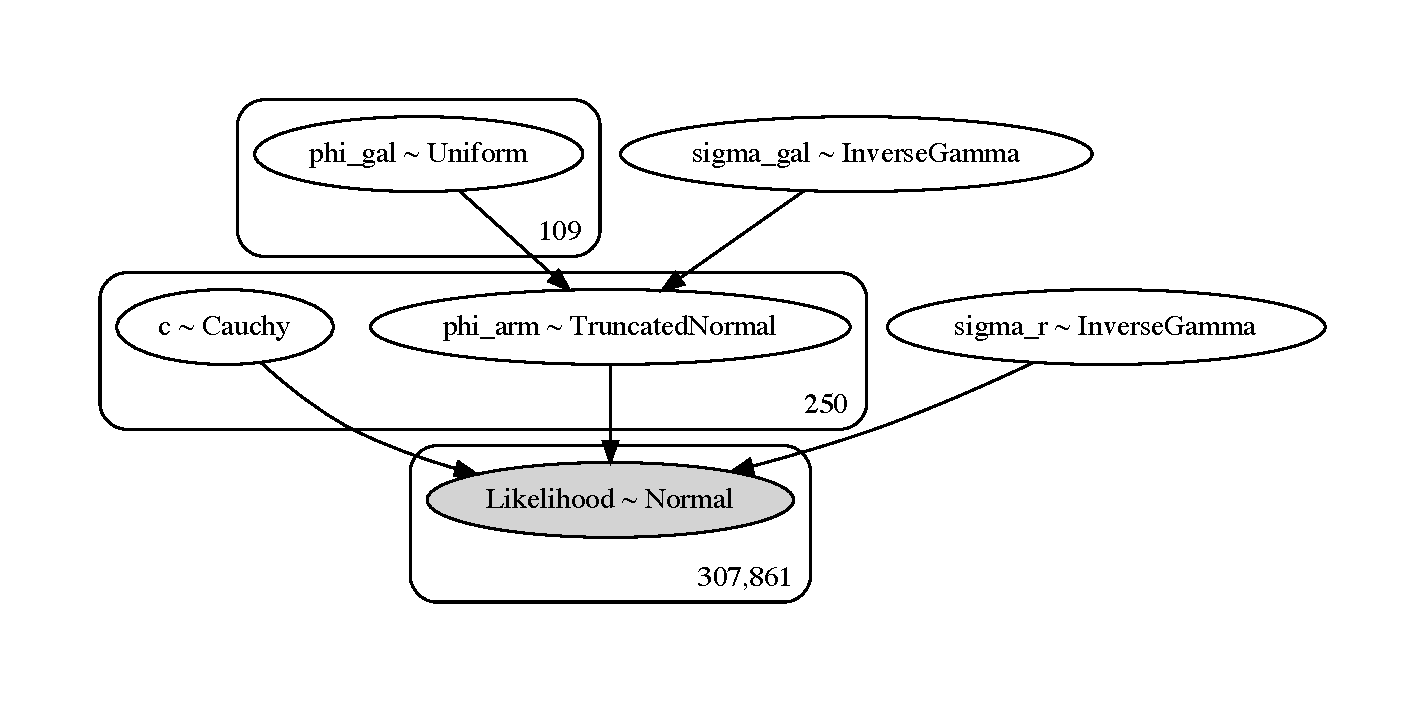
\includegraphics[width=8cm]{plots/plots_n109d1000t500/model.pdf}
%   \caption{The model used for galaxy pitch angle measurement for the sample.}
%   \label{fig:pymc3-model}
% \end{figure}

To perform inference, we make use of the No-U-Turn-Sampler (NUTS, \citealt{2011arXiv1111.4246H}), implemented in PYMC3\footnote{\url{https://docs.pymc.io/}}, an open source probabilistic programming framework written in python \citep{pymc3_paper}.
